% Three-state chain of the worked example. Rows sum to 1.
% P = [1/2 1/2 0; 1/3 1/3 1/3; 0 1/2 1/2].
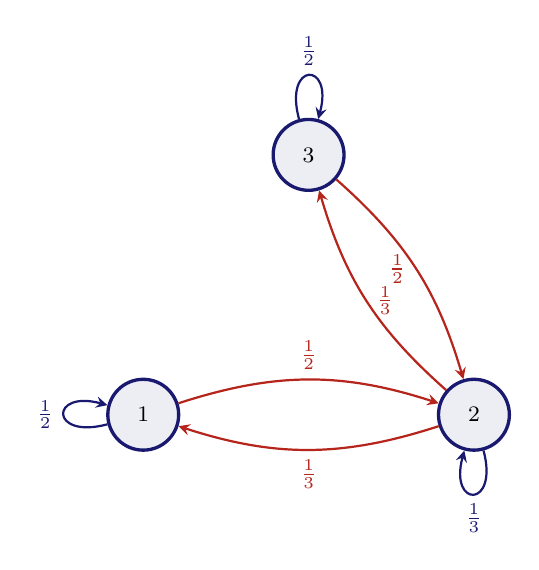
\begin{tikzpicture}[>=stealth,every node/.style={font=\footnotesize},st/.style={circle,draw=MidnightBlue,very thick,fill=MidnightBlue!8,minimum size=9mm}]
\node[st] (a) at (0,0) {$1$};
\node[st] (b) at (4.2,0) {$2$};
\node[st] (c) at (2.1,3.3) {$3$};
\draw[->,thick,BrickRed] (a) to[bend left=18] node[above] {$\frac12$} (b);
\draw[->,thick,BrickRed] (b) to[bend left=18] node[below] {$\frac13$} (a);
\draw[->,thick,BrickRed] (b) to[bend left=16] node[right] {$\frac13$} (c);
\draw[->,thick,BrickRed] (c) to[bend left=16] node[left] {$\frac12$} (b);
\draw[->,thick,MidnightBlue] (a) to[loop left,looseness=8] node[left] {$\frac12$} (a);
\draw[->,thick,MidnightBlue] (b) to[loop below,looseness=8] node[below] {$\frac13$} (b);
\draw[->,thick,MidnightBlue] (c) to[loop above,looseness=8] node[above] {$\frac12$} (c);
\end{tikzpicture}
